\section{Appendix: Equivalent Mass}
\label{app:Equivalent Mass Derivation}
This appendix outlines the calculations used to determine the equivalent mass of the measurement system. The equivalent mass is determined by analyzing the forces and moments acting on the system. The system is shown in Figure \ref{fig:Measurement System}.

A schematic of the measurement system is shown in Figure \ref{fig:Measurement System}. The equivalent mass of the system is given by
\begin{figure}[H]
    \centering
    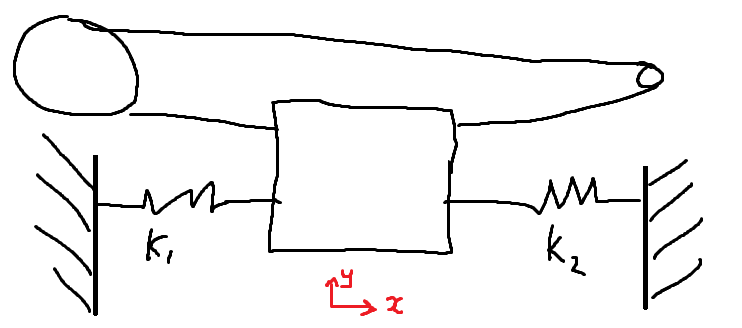
\includegraphics[width=0.5\textwidth]{Sections/Figures/system.png}
    \caption{Cart and Pulley Measurement System}
    \label{fig:Measurement System Appendix}
\end{figure}
\begin{figure}[h]
    \centering 
    \begin{minipage}{0.45\textwidth}
        \centering
        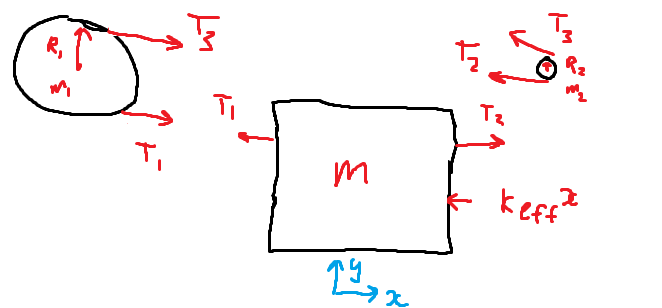
\includegraphics[width=0.9\textwidth]{Sections/Figures/fbd.png}
        \caption{Free Body Diagram of the Cart and Pulleys}
        \label{fig:Cart FBD Appendix}
    \end{minipage}\qquad
    \begin{minipage}{0.45\textwidth}
        \centering
        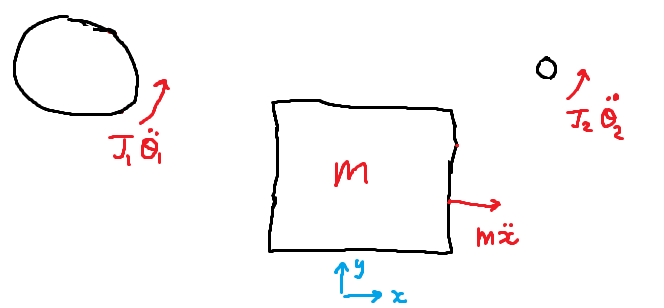
\includegraphics[width=0.9\textwidth]{Sections/Figures/mad.png}
        \caption{Mass Acceleration Diagram of the Cart and Pulleys}
        \label{fig:Cart MAD Appendix}
    \end{minipage}  
\end{figure}
Taking the sum of forces in $x$, the moment about pulley 1's and pulley's 2 mass center, 
\begin{align}
    \rightarrow \sum F_x &:= m_{\text{cart}} \ddot{x} \nonumber \\
    &=  T_2 - T_1 - k_{\text{eff}}x \label{eq:Cart Force in x Appendix} \\
    \circlearrowleft \sum M_{\text{pulley 1}} &:= J_1 \ddot{\theta}_1 \nonumber \\
    &= r_1 (T_1 - T_3) \label{eq:Pulley 1 Moment Appendix} \\
    \circlearrowleft \sum M_{\text{pulley 2}} &:= J_2 \ddot{\theta}_2 \nonumber \\
    &= r_2 (T_3 - T_2) \label{eq:Pulley 2 Moment Appendix}
\end{align}
Assuming the cable does not slip in the the grooves of the pulleys at radius $r_1$ and $r_2$,
\begin{align}
    \theta_1 &= \frac{\ddot{x}}{r_1}, \quad \theta_2 = \frac{\ddot{x}}{r_2} \label{eq:Kinematic pure rotation for theta1 and theta2 Appendix}
\end{align}

% From the Section \ref{sec:Equivalent Mass}, the equations from summing the forces in the x and the moment about pulley 1's and pulley's 2 mass center are described by Eq. (\ref{eq:Cart Force in x}), (\ref{eq:Pulley 1 Moment}), and (\ref{eq:Pulley 2 Moment}). Assuming the cable does not slip, the kinematic relationship for the pulleys is given by Eq. (\ref{eq:Kinematic pure rotation for theta1 and theta2}). The moment of inertia of the pulleys is given by Eq. (\ref{eq:Moment of Inertia of Pulleys}).

% Next, applying Eq. (\ref{eq:Moment of Inertia of Pulleys}) and Eq. (\ref{eq:Kinematic pure rotation for theta1 and theta2}) to Eq. (\ref{eq:Pulley 1 Moment}) and Eq. (\ref{eq:Pulley 2 Moment}), we get
Next, combining Eq. (\ref{eq:Cart Force in x Appendix}), (\ref{eq:Pulley 1 Moment Appendix}), (\ref{eq:Pulley 2 Moment Appendix}) and using Eq. (\ref{eq:Kinematic pure rotation for theta1 and theta2 Appendix}), we get
\begin{align}
    J_1 \frac{\ddot{x}}{r_1} &= r_1 (T_1 - T_3) \nonumber \\
    \implies \frac{J_1}{r_1^2} \ddot{x} &= T_1 - T_3 \label{eq:Pulley 1 Moment Simplified Appendix} \\
    J_2 \frac{\ddot{x}}{r_2} &= r_2 (T_3 - T_2) \nonumber \\
    \implies \frac{J_2}{r_2^2} \ddot{x} &= T_3 - T_2 \label{eq:Pulley 2 Moment Simplified Appendix}
\end{align}
Performing Eq. (\ref{eq:Pulley 1 Moment Simplified Appendix}) + Eq. (\ref{eq:Pulley 2 Moment Simplified Appendix}) gives
\begin{align}
    \frac{J_1}{r_1^2} \ddot{x} + \frac{J_2}{r_2^2} \ddot{x} &= T_1 - T_3 + T_3 - T_2 \nonumber \\
    \frac{J_1}{r_1^2} \ddot{x} + \frac{J_2}{r_2^2} \ddot{x} &= T_1 - T_2 \label{eq:Pulley 1 and 2 Combined Simplified 1 Appendix}
\end{align}
And Eq. (\ref{eq:Pulley 1 and 2 Combined Simplified 1 Appendix}) + Eq. (\ref{eq:Cart Force in x Appendix}) gives
\begin{align}
    % \left(m + \frac{m_1 R_1^2}{2 r_1^2} + \frac{m_2 R_2^2}{2 r_2^2}\right) \ddot{x} &= T_1 - T_2 - T_1 + T_2 - k_{\text{eff}}x \nonumber 
    \left(m + \frac{J_1}{r_1^2} + \frac{J_2}{r_2^2}\right) \ddot{x} &= - k_{\text{eff}}x \label{eq:Equivalent Mass Equation of Motion Simplified Appendix}
\end{align}
Finally,
\begin{empheq}[box=\fbox]{align}
    \underbrace{\left(m_{\text{cart}} + \frac{J_1}{r_1^2} + \frac{J_2}{r_2^2}\right)}_{m_e} \ddot{x} + k_{\text{eff}}x = 0 \label{eq:General Equivalent Mass Equation of Motion Appendix}
\end{empheq}
If the pulleys are assumed to be uniform disks,
\begin{align}
    J_1 &= \frac{1}{2} m_{1} r_1^2, \quad J_2 = \frac{1}{2} m_{2} r_2^2 \label{eq:Moment of Inertia of Pulleys Appendix}
\end{align}
Substituting Eq. (\ref{eq:Moment of Inertia of Pulleys Appendix}) into Eq. (\ref{eq:General Equivalent Mass Equation of Motion Appendix}) gives
\begin{empheq}[box=\fbox]{align}
    % \left(m_{\text{cart}} + \frac{1}{2} m_{1} + \frac{1}{2} m_{2}\right) \ddot{x} + k_{\text{eff}}x = 0 \label{eq:Equivalent Mass Equation of Motion Appendix}
    \underbrace{\left(m_{\text{cart}} + \frac{1}{2} m_{1} + \frac{1}{2} m_{2}\right)}_{m_e} \ddot{x} + k_{\text{eff}}x = 0 \label{eq:Equivalent Mass Equation of Motion Appendix}
\end{empheq}
In actuality, the equivalent mass in (\ref{eq:Equivalent Mass Equation of Motion Appendix}) should be larger than (\ref{eq:General Equivalent Mass Equation of Motion Appendix}) since the pulleys aren't uniform disks due to the groove.